\subsection{zigzag}

Now we've got a 8x8 matrix.
We can convert it into a 1D array by using the zigzag pattern.

\begin{figure}[H]
    \centering
    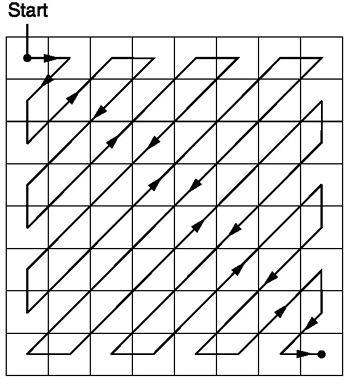
\includegraphics[width=0.3\textwidth]{src/assets/zigzag.jpg}
    \caption{Zigzag pattern}
    \label{fig:zigzag}
\end{figure}

\cFF{src/part-02/assets/zigzag.py}{Zigzag}{zigzag}

\subsection{Run length encoding}
With all this, we've got a lot of zeros at the end of the vector.
So we can implement a run length encoding to save some space.

\cFF{src/part-02/assets/rle.py}{Run length encoding}{run_length_encoding}

\subsection{Huffman coding}

Ok, it is the final step.
Before digging into the Huffman coding, let's sum up what we've done so far.


\begin{figure}[H]
    \centering
    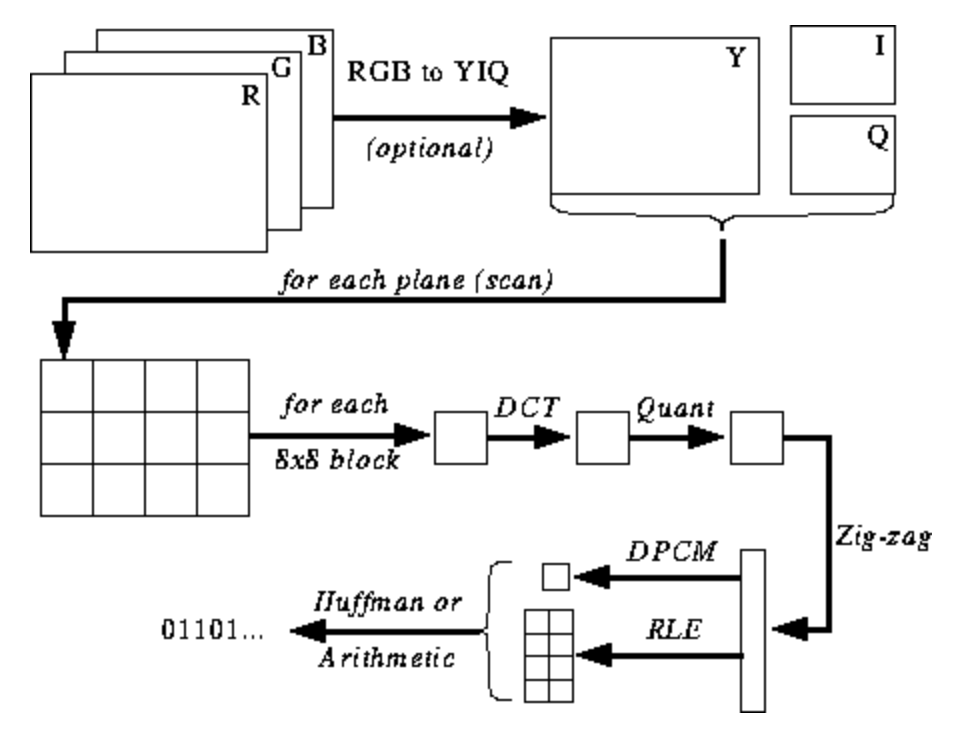
\includegraphics[width=0.5\textwidth]{src/assets/encoding.png}
    \caption{JPEG compression}
    \label{fig:encoding}
\end{figure}

Figure \ref{fig:encoding} is from \href{https://users.cs.cf.ac.uk/Dave.Marshall/Multimedia/node234.html}{Dave Marshall's website}.
From the zigzag pattern, it is lossless compression. It is reshaping data with some
math (to put it simply).
After doing that, we'll have to save the data in a binary file.
For this, I followed the all \href{https://yasoob.me/posts/understanding-and-writing-jpeg-decoder-in-python}{tuto} to decode en JPEG image.
But it is low level, byte reading and writing, and even if I make it works on some
images, it doesn't work all the time.
\textbf{So I preferred begin the decoding algorithm from this point} (before the zigzag).


